\chapter{Background}

\section{Definitions}
This section covers and differentiates between the basic non-mathematical definitions and terms used in this thesis.

\subsection{Virtual and augmented reality}\label{sec:VAR}
The words virtual reality (VR) and augmented reality (AR) can be constantly read in the recent news all over the internet and other media. However, they are used in various contexts and are often defined differently. The definition used in this thesis is therefore only one small aspect of the whole field and should help to differentiate between the two concepts. 
\subsubsection{Virtual reality}
Virtual reality\index{Virtual reality} can be defined as \enquote{an electronic simulation in which images are generated in real time (...) from a stored database and displayed in such a way as to facilitate real-time interaction with the database (...).} \cite[p.148]{Latham.1995}

A virtual reality application uses a combination of software and hardware to let the user experience immersion, interaction and imagination (the three I's of virtual reality) in a virtual world. Whereas the first two I's should be clear and understandable, the last one is often underrated or even left out. Since virtual reality only counts on virtual content and given the fact that computer graphics are still not a perfect representation of our \enquote{reality}, the user's imagination is a very important aspect of an application (\cite[p.3 et seq.]{Burdea.2003}).

Typically, a common computer game can not be classified as a virtual reality application unless it includes the collection and usage of other data than only the keyboard and mouse inputs. For this purpose, a VR application often comes with other interfaces such as a head-mounted display (HMD)\index{Head-mounted display} \footnote{The idea of a HMD started with Morton Heilig's  \index{Morton L. Heilig} U.S. patent in 1960 (see \cite{Heilig.1957}). Recent popular models include the \textit{Oculus Rift} (see \cite{Oculus.2016})\index{Head-mounted display!Oculus Rift} and \textit{Google Cardboard} (see \cite{GoogleDev.2016})\index{Head-mounted display!Google Cardboard}. The HMD tracks, amongst other things, the head position and its movement and displays the stereo image.}. An imaginary example for a perfect virtual reality environment is Star Trek's Holodeck, as mentioned before (\autoref{sec:preface}).

\subsubsection{Augmented reality}
\begin{figure}[htbp]
		\centering
		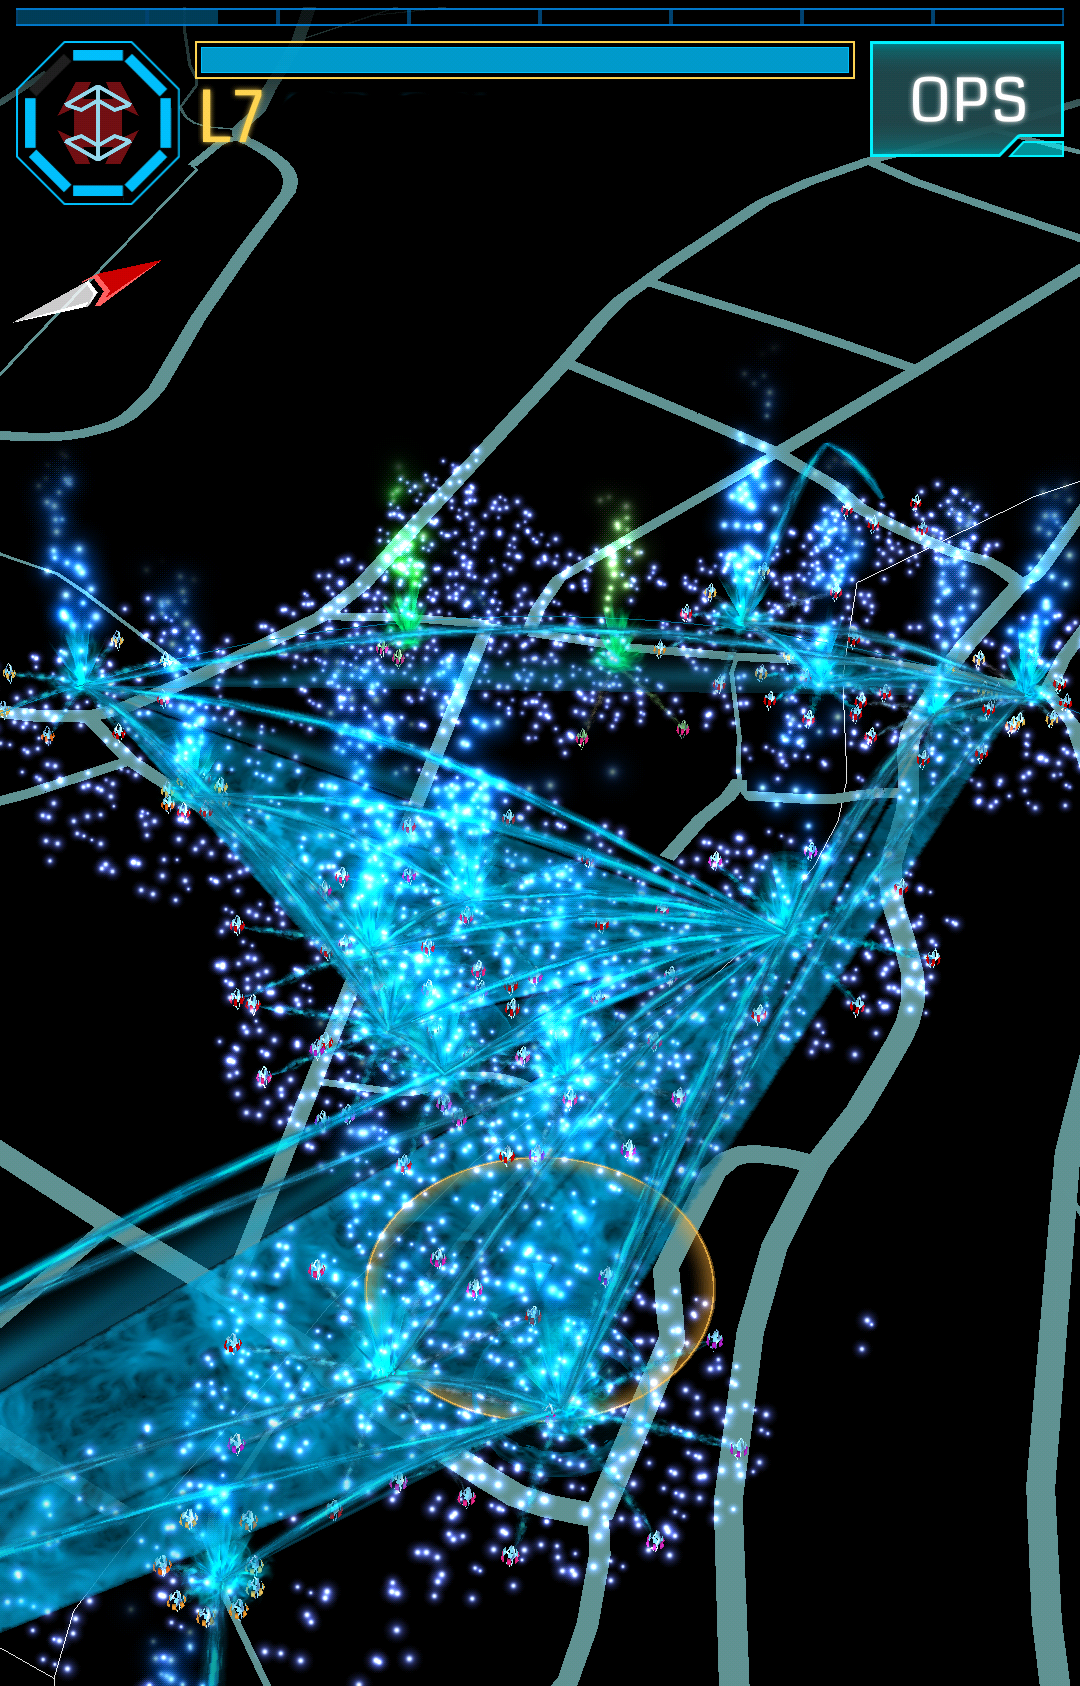
\includegraphics[width=0.4\textwidth]{figures/Ingress}
		\caption[Screenshot of the mobile AR game Ingress]{Screenshot of the mobile AR game Ingress showing the portals around the Hochschule Furtwangen University (\textit{source:} \cite{Haefele.2014}).}
		\label{fig:Ingress}
\end{figure}
In comparison to virtual reality, augmented reality \index{Augmented reality} extends our \enquote{real world} with virtual (digital) content, which must be embedded seamlessly to provide a fully immersive experience. The users can interact with virtual objects and can be provided with relevant additional information about their environment. The virtual data is computed in real-time and is displayed as an overlay on top of the \enquote{real world} in front of the user's eyes. AR highly relies on its technologies. Relevant topics, amongst others, are object recognition, location tracking, interfaces\footnote{A common interface for AR was and still is the head-up display (HUD)\index{Head-up display}, often used for military application (see \cite[p.6]{Burdea.2003}). But also immaterial displays, such as fog screens, are researched (see \cite[p.25 et seq.]{Toennis.2010}).} and real-time computation (compare with \cite[p.1 et seqq.]{Toennis.2010}). 

The game \textit{Ingress}\index{Ingress} by \textit{Niantic, Inc.} (see \autoref{fig:Ingress} for a screenshot), in which two factions fight over virtual portals, is an example for a location-based mobile AR game. The portals, which are linked to real places all over the world, and other game functions are displayed on the user's mobile device in real-time. The users travel to these real places to conquer or defend the portals in the name of their faction (\cite{Niantic.2016}). 

\subsection{Computer vision}\label{ssec:cv}
\todo{multiple view geometry? stereo vision?}
\index{Computer vision} \index{Stereo vision}

David Lowe: \enquote{Computer vision (also often referred to as "machine vision" for industrial vision applications) is the automated extraction of information from images. This differs from image processing, in which an image is processed to produce another image. This page covers only products based on computer vision, and it does not cover image processing or any of the many suppliers of sensors or other equipment to the industry.} (\cite{Lowe.2016})

\section{History}\label{sec:history}
\subsection{First developments}
In the late 50s of the 19th century \textit{Morton Leonard Heilig}\index{Morton L. Heilig} dreamed about the revolution of cinematic story telling and designed with his \enquote{stereoscopic-television apparatus for individual use}\index{Head-mounted display!Stereoscopic-television apparatus for individual use} the first head-mounted display (see \autoref{fig:Heilig}). The helmet was planned to display stereoscopic images, play surround sound and even add smell to the sensory experience, but was never actual built. His ideas were ahead of their time and could not yet be realized with the technology of the time (compare with \cite[p.3]{Toennis.2010} and \cite[p.4 et seq.]{Burdea.2003}). 

In the decades to follow, several attempts to bring input and display devices for virtual reality onto the consumer market failed due to their high costs and their lack of software. In 1992, \textit{Jaron Lanier}\index{Jaron Lanier} and his company \textit{VPL Research} released the \textit{DataGlove}\footnote{The \textit{datagloves}\index{Dataglove} (also called \textit{wire-} or \textit{cybergloves}) are another step into more immersive input devices, since hand gestures can be directly used to interact with the virtual world.}\index{Dataglove!DataGlove} at the unaffordable prize point of \$9000 USD. The low number of games for \textit{Nintendo's} cheaper \textit{PowerGlove}\index{Dataglove!PowerGlove} led to its discontinuation in 1993 soon after its introduction (\cite[p.8 et seq.]{Burdea.2003} and \cite[p.19 et seq.]{Doerner.2013}).

\begin{figure}[htbp]
		\centering
		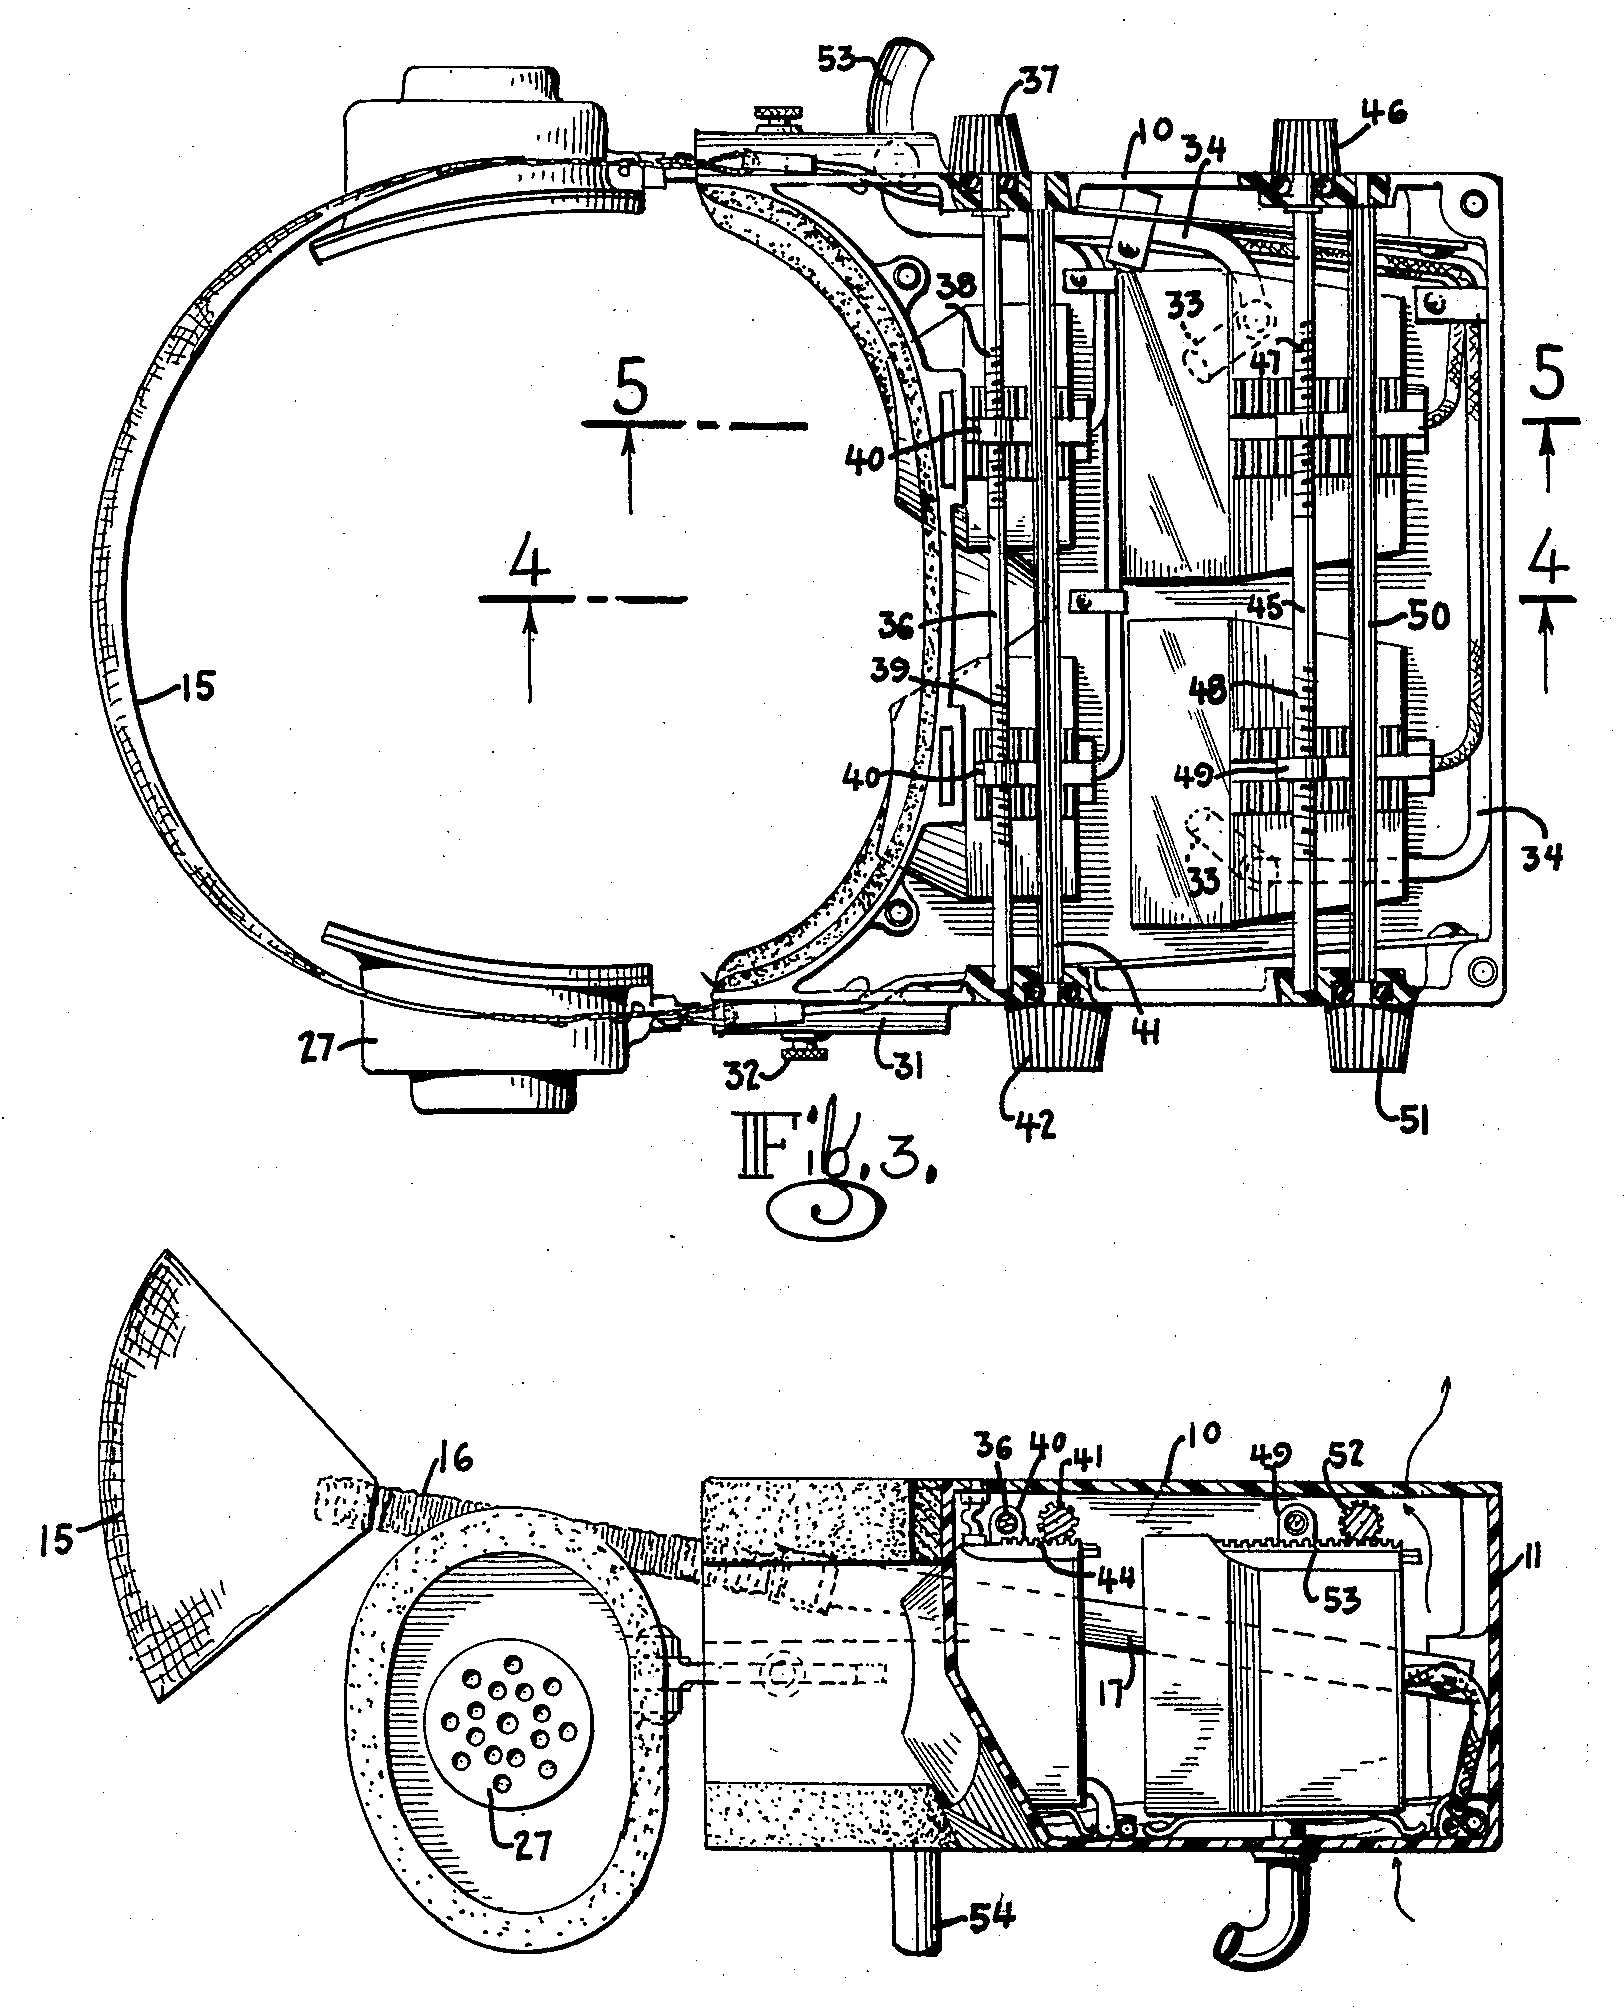
\includegraphics[width=0.4\textwidth]{figures/Heilig_HMD}
		\caption[Stereoscopic-television apparatus for individual use]{Morton Heilig's stereoscopic-television apparatus for individual use (\textit{source: \cite{Heilig.1957}}).}
		\label{fig:Heilig}
\end{figure}

\subsection{Disappointments}
The 80s and 90s were characterized by heavily marketed products, that ultimately disappointed the users and failed to live up to the \enquote{mediahype}. The expectations for virtual reality applications were too high and the technological development was not fast enough. The hardware was too costly\footnote{The fastest graphics system, the \textit{Reality Engine} by \textit{Silicon Graphics}, cost \$100,000 USD at its release in the 1990s(\cite[p.10]{Burdea.2003}).}, the market for VR was too small and there were no investment funds available for companies. These deficits led to the bankruptcy of many companies and caused a serious crisis for the VR industry (\cite[p.10]{Burdea.2003}). 

\todo{spell-check from here}
Meanwhile the development of virtual reality \todo{... the role of military and NASA, sensor improvement, ...} \\

With the improvement of computer hardware in the late 90s, the graphics computation began to meet the requirements for VR and the hardware was finally affordable for consumers (\cite[p.10 et seq.]{Burdea.2003}, \cite{Doerner.2013} and \cite[p.3]{Toennis.2010}).

\subsection{Today's usage of computer vision}\label{ssec:Today}
Fortunately, recent successes in the industry were made and the computer vision plays an increasing role in many fields. \textit{David Lowe}, Senior Research Scientist at Google Seattle, has enlisted the following categories of today's important industrial applications of computer vision\footnote{Although he states that his list is not complete and not up-to-date, it can be used as an overview. Go to his homepage to read more about specific applications: \cite{Lowe.2016}} (freely adapted from \cite{Lowe.2016}): 

\begin{description}
\item [Automotive driver assistance and traffic management,]\hfill \\ such as warning vision systems and real-time traffic management.
\item [Eye and head tracking,]\hfill \\ which is also included in head-mounted displays.
\item [Film and video,]\hfill \\ e.g. tracking of the ball in sports for sport-analyzing or motion tracking systems for animated movies \todo{maybe cite PETER and ALEX}.
\item [Gesture recognition,]\hfill \\ such as full-body motion sensing with the Mircosoft Kinect and gesture recognition as computer inputs for gaming or other computer-related activities.
\item [Industrial automation and inspection,]\hfill \\ like systems for inspection and process control in the electronic or food and agriculture industry. 
\item [Medical and biomedical,]\hfill \\ e.g. the detection and tracking of markers in real-time stereo vision for surgeons.
\item [Object recognition and AR for mobile devices,]\hfill \\ including real-time product recognition and image refinement applications, such as face-swapping apps.
\item [Photography,]\hfill \\ e.g. automated panorama stitching for multiple images.
\item [Safety monitoring,]\hfill \\ monitoring of areas to warn of accidents, e.g. in swimming pools.
\item [Security and biometrics,]\hfill \\ detection and counting of people for security purposes, fingerprint or license plate recognition.
\item [3D modeling,]\hfill \\ 3D scanners of objects or the 3D reconstruction from a number of photographs. 
\item [Web and cloud applications,]\hfill \\ such as image retrieval based on content. 
\end{description}

Regarding all these examples, the entertainment industry seems to be the slowest candidate, which is partly owed to its users high expectations regarding the (graphics) quality. 
